\documentclass[border=0pt,10pt]{standalone}
\usepackage[T1]{fontenc}
\usepackage{lmodern}
\usepackage{pgfplots}
\pgfplotsset{compat=1.17}
\usepgfplotslibrary{groupplots}
\usepackage{xcolor}
\definecolor{oi-blue}{HTML}{0072B2}
\definecolor{oi-vermillion}{HTML}{D55E00}
\definecolor{oi-green}{HTML}{009E73}
\definecolor{oi-purple}{HTML}{CC79A7}
\definecolor{oi-black}{HTML}{000000}
% semantic_sha256: bd2a953e6fdeba82f892112e77e569b479863bd0d1672a21f119ca1f80c333bc
\begin{document}
\begin{minipage}{181.86mm}
\centering
{\bfseries\fontsize{10}{12}\selectfont PP-U-SG | D1 | final\_refit}\\[2mm]
{\fontsize{8}{10}\selectfont planned=42, monitored=42, missing-history=0, status=complete\_history\_coverage}\\[3mm]
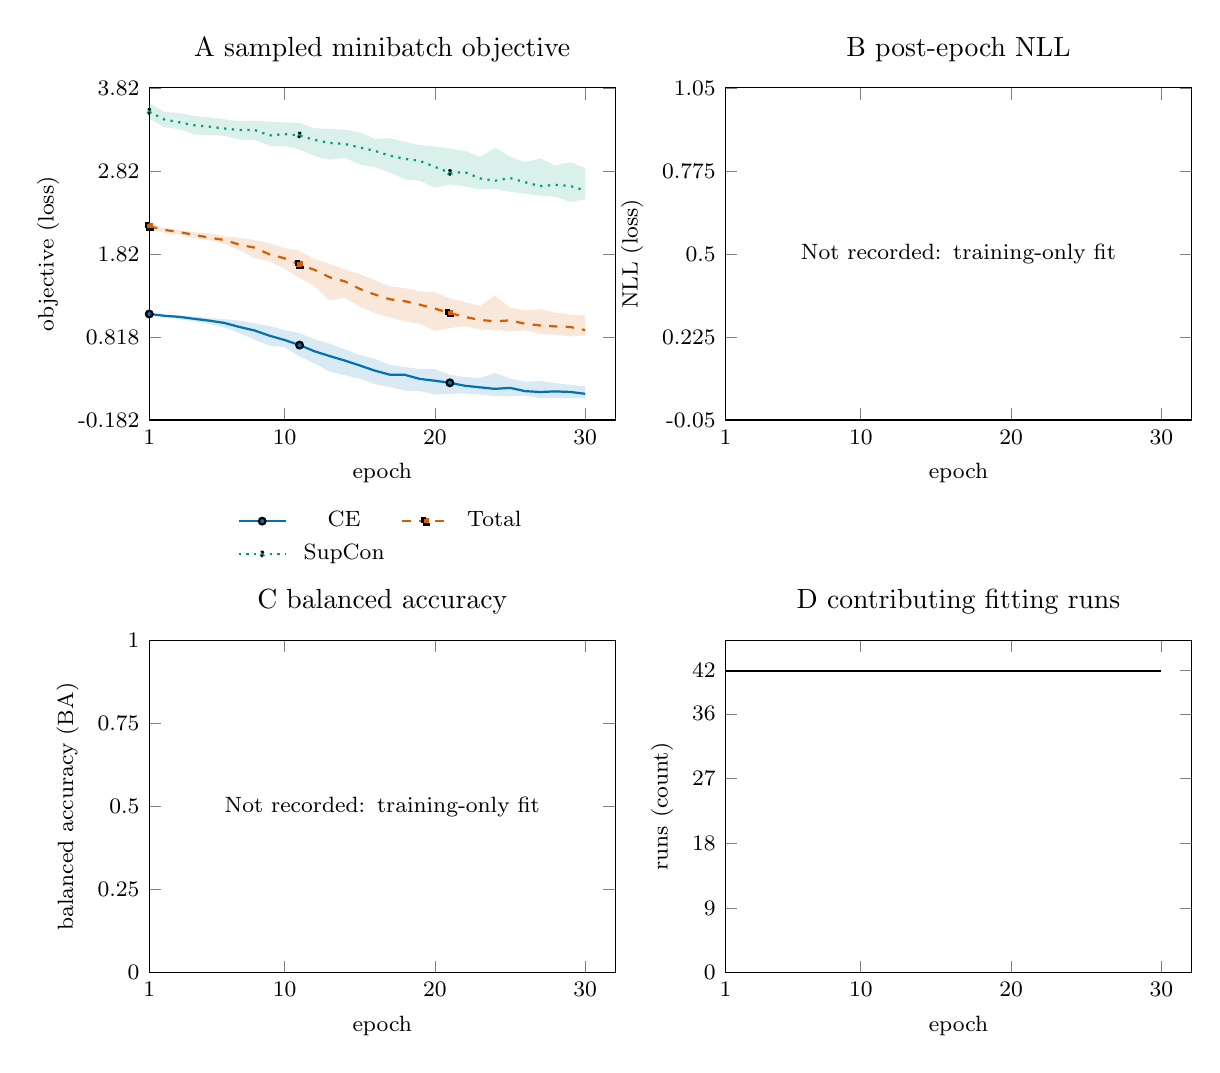
\begin{tikzpicture}
\begin{groupplot}[group style={group size=2 by 2, horizontal sep=14mm, vertical sep=28mm}]
\nextgroupplot[width=75mm, height=58mm, title={A sampled minibatch objective}, xlabel={epoch}, ylabel={objective (loss)}, xmin=1, xmax=32, xtick={1,10,20,30}, ymin=-0.18180758893489837, ymax=3.8179593676328656, ytick={-0.18180758893489837,0.81813415020704261,1.8180758893489835,2.8180176284909244,3.8179593676328656}, yticklabels={-0.182,0.818,1.82,2.82,3.82}, tick label style={font=\fontsize{8}{9}\selectfont, text=black}, label style={font=\fontsize{8}{9}\selectfont, text=black}, title style={font=\fontsize{10}{11}\selectfont, text=black}, legend style={at={(0.5,-0.24)},anchor=north,draw=none,fill=none,font=\fontsize{8}{9}\selectfont,row sep=1pt,column sep=4pt,legend columns=2}]
\addplot[fill=oi-blue,opacity=0.15,draw=none,forget plot] coordinates {(1,1.0856326937675476) (2,1.0598683416843415) (3,1.0317184537649156) (4,1.0076779574155807) (5,0.97418075352907185) (6,0.93077768981456754) (7,0.86571775227785108) (8,0.78542925715446477) (9,0.71282804310321812) (10,0.69732655286788936) (11,0.58303825557231903) (12,0.49919560104608535) (13,0.40115770623087887) (14,0.35744420737028121) (15,0.31809508465230468) (16,0.25017666742205624) (17,0.21648794487118722) (18,0.17275145836174491) (19,0.1673478651791811) (20,0.12504655588418245) (21,0.13377721048891544) (22,0.13824292793869972) (23,0.12551980316638947) (24,0.10585156846791506) (25,0.10695114862173796) (26,0.11149870119988918) (27,0.081640640459954741) (28,0.084256971068680284) (29,0.078249969286844134) (30,0.078303194977343088) (30,0.22592099495232104) (29,0.24151559174060822) (28,0.26305673867464058) (27,0.2883186027407646) (26,0.27843546681106091) (25,0.31980964653193944) (24,0.38531484417617318) (23,0.32291662804782389) (22,0.33552989736199379) (21,0.36268689185380937) (20,0.43330932110548015) (19,0.43253118991851802) (18,0.4561954692006111) (17,0.48170630931854247) (16,0.5557661600410938) (15,0.60191672295331955) (14,0.66910101026296609) (13,0.73877602815628052) (12,0.79127880483865742) (11,0.86360255926847451) (10,0.90232046246528619) (9,0.94998932182788853) (8,0.98391022831201558) (7,1.015876193344593) (6,1.0319342195987702) (5,1.0506824672222137) (4,1.0617280423641204) (3,1.0772065997123719) (2,1.0881578236818314) (1,1.1016241073608399)};
\addplot[color=oi-blue, mark=*, mark options={draw=black}, mark repeat=10, mark size=1.2pt, solid, line width=0.8pt] coordinates {(1,1.0949308127164841) (2,1.073481485247612) (3,1.0606247633695602) (4,1.0368818044662476) (5,1.0149508118629456) (6,0.98706588894128799) (7,0.93911905586719513) (8,0.89673701673746109) (9,0.83387202769517899) (10,0.78211869299411774) (11,0.7205837145447731) (12,0.64555593580007553) (13,0.58850418031215668) (14,0.5350494384765625) (15,0.47544250264763832) (16,0.41320693865418434) (17,0.36464813351631165) (18,0.36279672011733055) (19,0.31336186826229095) (20,0.29134860634803772) (21,0.26664446480572224) (22,0.23052096273750067) (23,0.21220794506371021) (24,0.19345081597566605) (25,0.20562633499503136) (26,0.16615965217351913) (27,0.15593144204467535) (28,0.16270777862519026) (29,0.15640896093100309) (30,0.13411116786301136)};
\addlegendentry{CE}
\addplot[fill=oi-vermillion,opacity=0.15,draw=none,forget plot] coordinates {(1,2.1270623743534087) (2,2.0735590636730192) (3,2.0522856354713439) (4,2.01012806892395) (5,1.9851469248533249) (6,1.9387914001941682) (7,1.8650114387273788) (8,1.7704753756523133) (9,1.7264228612184525) (10,1.6421109914779664) (11,1.5285637527704239) (12,1.4299254626035691) (13,1.258315172791481) (14,1.2900392413139343) (15,1.1868747889995575) (16,1.1080580115318299) (17,1.056646180152893) (18,1.0060530707240105) (19,0.9771742627024651) (20,0.89188452214002611) (21,0.92636079490184786) (22,0.94793632179498677) (23,0.90837612003087997) (24,0.90391840338706975) (25,0.88492824137210846) (26,0.89917314946651461) (27,0.85227024406194685) (28,0.84762542545795438) (29,0.82466221153736119) (30,0.83917159736156466) (30,1.0799720555543899) (29,1.0892047673463821) (28,1.1108155593276023) (27,1.1545918136835098) (26,1.136691190302372) (25,1.1722286671400071) (24,1.3163785859942436) (23,1.1937988549470901) (22,1.238493025302887) (21,1.2859250277280807) (20,1.358028593659401) (19,1.3688625514507293) (18,1.4059059292078018) (17,1.4292267382144928) (16,1.5000525444746018) (15,1.5762408256530762) (14,1.6316047072410582) (13,1.6973439455032349) (12,1.7570473313331605) (11,1.8565720111131667) (10,1.8893032729625703) (9,1.9469787180423737) (8,1.9862539261579513) (7,2.0119742006063461) (6,2.0306149214506148) (5,2.0667977690696717) (4,2.079546296596527) (3,2.1048877775669097) (2,2.1302009463310241) (1,2.1894751131534576)};
\addplot[color=oi-vermillion, mark=square*, mark options={draw=black}, mark repeat=10, mark size=1.2pt, dashed, line width=0.8pt] coordinates {(1,2.1515755951404572) (2,2.1086755394935608) (3,2.0810527205467224) (4,2.0475934743881226) (5,2.0141947865486145) (6,1.9861680716276169) (7,1.9302371442317963) (8,1.8944440633058548) (9,1.8131558299064636) (10,1.7661450058221817) (11,1.6907245963811874) (12,1.6262165158987045) (13,1.5373400002717972) (14,1.4885440468788147) (15,1.3978370875120163) (16,1.3299925029277802) (17,1.2724762856960297) (18,1.2495038509368896) (19,1.2067659944295883) (20,1.1598669588565826) (21,1.1066138297319412) (22,1.0599350258708) (23,1.0233452767133713) (24,1.0071079283952713) (25,1.0177947655320168) (26,0.97765515744686127) (27,0.95736580342054367) (28,0.94625527411699295) (29,0.93861094117164612) (30,0.90205781906843185)};
\addlegendentry{Total}
\addplot[fill=oi-green,opacity=0.15,draw=none,forget plot] coordinates {(1,3.4479358553886414) (2,3.3453033924102784) (3,3.3221079468727113) (4,3.2552877068519592) (5,3.2511464059352875) (6,3.2410943746566772) (7,3.1964386940002441) (8,3.1896918296813963) (9,3.1205473363399507) (10,3.1201577365398405) (11,3.077597051858902) (12,2.9956335783004762) (13,2.952390158176422) (14,2.9759127616882326) (15,2.8959322690963747) (16,2.8622034549713136) (17,2.8003610849380491) (18,2.7182777404785154) (19,2.6979567289352415) (20,2.6171509385108949) (21,2.6555216312408447) (22,2.6293771326541902) (23,2.5976445138454438) (24,2.6001268684864045) (25,2.5663397192955015) (26,2.5443472623825074) (27,2.5197111427783967) (28,2.5071624875068665) (29,2.4464902639389039) (30,2.4765081226825716) (30,2.852531063556671) (29,2.9234360575675962) (28,2.8823953330516816) (27,2.970321273803711) (26,2.9218943476676942) (25,2.9887548148632046) (24,3.0980372369289397) (23,2.9863054692745208) (22,3.0601274371147156) (21,3.084771341085434) (20,3.1125260949134828) (19,3.1284343004226685) (18,3.1693657636642456) (17,3.2126692116260527) (16,3.2056096255779267) (15,3.2809747159481049) (14,3.3146156489849092) (13,3.3242769181728362) (12,3.3323620378971102) (11,3.39392951130867) (10,3.4022493064403534) (9,3.4091544330120085) (8,3.4235895216464995) (7,3.4179696142673492) (6,3.4393733561038973) (5,3.4634745717048645) (4,3.4785381197929381) (3,3.5159092068672182) (2,3.5291576981544495) (1,3.6361517786979674)};
\addplot[color=oi-green, mark=triangle*, mark options={draw=black}, mark repeat=10, mark size=1.2pt, dotted, line width=0.8pt] coordinates {(1,3.5302964150905609) (2,3.4375616908073425) (3,3.4030961394309998) (4,3.3672485649585724) (5,3.3511452674865723) (6,3.3282173275947571) (7,3.3103492558002472) (8,3.3126080334186554) (9,3.2449243068695068) (10,3.2617180645465851) (11,3.2451300323009491) (12,3.1912077367305756) (13,3.15482297539711) (14,3.143012672662735) (15,3.1005450189113617) (16,3.0600780248641968) (17,3.0007161200046539) (18,2.9641488194465637) (19,2.9379274249076843) (20,2.8670656383037567) (21,2.7938806414604187) (22,2.8038811683654785) (23,2.7281034588813782) (24,2.6991403698921204) (25,2.7324970662593842) (26,2.6822158992290497) (27,2.6342768967151642) (28,2.6504969596862793) (29,2.6366429328918457) (30,2.5817576944828033)};
\addlegendentry{SupCon}
\nextgroupplot[width=75mm, height=58mm, title={B post-epoch NLL}, xlabel={epoch}, ylabel={NLL (loss)}, xmin=1, xmax=32, xtick={1,10,20,30}, ymin=-0.050000000000000003, ymax=1.05, ytick={-0.050000000000000003,0.22500000000000003,0.5,0.77500000000000002,1.05}, yticklabels={-0.05,0.225,0.5,0.775,1.05}, tick label style={font=\fontsize{8}{9}\selectfont, text=black}, label style={font=\fontsize{8}{9}\selectfont, text=black}, title style={font=\fontsize{10}{11}\selectfont, text=black}]
\node[align=center, text width=55mm, font=\fontsize{8}{9}\selectfont] at (axis cs:16.5,0.5) {Not recorded: training-only fit};
\nextgroupplot[width=75mm, height=58mm, title={C balanced accuracy}, xlabel={epoch}, ylabel={balanced accuracy (BA)}, xmin=1, xmax=32, xtick={1,10,20,30}, ymin=0, ymax=1, ytick={0,0.25,0.5,0.75,1}, yticklabels={0,0.25,0.5,0.75,1}, tick label style={font=\fontsize{8}{9}\selectfont, text=black}, label style={font=\fontsize{8}{9}\selectfont, text=black}, title style={font=\fontsize{10}{11}\selectfont, text=black}]
\node[align=center, text width=55mm, font=\fontsize{8}{9}\selectfont] at (axis cs:16.5,0.5) {Not recorded: training-only fit};
\nextgroupplot[width=75mm, height=58mm, title={D contributing fitting runs}, xlabel={epoch}, ylabel={runs (count)}, xmin=1, xmax=32, xtick={1,10,20,30}, ymin=0, ymax=46.200000000000003, ytick={0,9,18,27,36,42}, yticklabels={0,9,18,27,36,42}, tick label style={font=\fontsize{8}{9}\selectfont, text=black}, label style={font=\fontsize{8}{9}\selectfont, text=black}, title style={font=\fontsize{10}{11}\selectfont, text=black}]
\addplot[color=oi-black, solid, line width=0.8pt] coordinates {(1,42) (2,42) (3,42) (4,42) (5,42) (6,42) (7,42) (8,42) (9,42) (10,42) (11,42) (12,42) (13,42) (14,42) (15,42) (16,42) (17,42) (18,42) (19,42) (20,42) (21,42) (22,42) (23,42) (24,42) (25,42) (26,42) (27,42) (28,42) (29,42) (30,42)};
\end{groupplot}
\end{tikzpicture}
\par\vspace{6mm}
\begin{minipage}{175mm}
{\fontsize{8}{10}\selectfont RQ-S01 / Scope E: descriptive training diagnostics. 400-1800 cm-1 inputs: SG uses impulse replacement and Savitzky-Golay smoothing; arPLS uses impulse replacement and baseline correction; both finish with [0,1] min-max scaling. CE = chemical cross-entropy; SupCon = supervised contrastive; Paired = paired consistency; NLL = negative log-likelihood; BA = balanced accuracy. Authenticated complete monitor histories aggregated across unique fitting jobs into descriptive policy/recipe/stage curves. Curves summarize per-epoch minibatch-weighted training chemical cross-entropy and the composite total optimization objective; these sampled minibatch objectives differ from post-epoch evaluation negative log-likelihood. Auxiliary supcon/paired loss components are recipe-specific and are not directly comparable to the total objective across recipes. Validation metrics are recorded for source\_fit runs only and never substitute for a held-out test set; calibration\_model\_fit and final\_refit rows carry training-only diagnostics. Source\_fit optimization uses a 30-epoch minimum stopping threshold and a 200-epoch maximum; refit stages reuse the caller-selected duration. Curves are fitting-run-weighted descriptive summaries over correlated runs (seeds/splits). Lines show medians; 10th/90th percentiles describe variation among saved fitting runs, not confidence intervals. Only runs that reached each epoch contribute; early stopping changes the composition, and stopped runs are not carried forward. Fitting jobs are not independent chemical samples: the dataset has 598 spectra from 69 physical samples and 10 instruments. Coverage is limited to saved SG/arPLS monitor histories; historical MIN losses are not pooled or invented. A missing history is not a zero loss or proof of a failed model. These curves do not support hypothesis tests, superiority claims, model selection, or new uncertainty inference. P08 learned-method performance is reported elsewhere.}
\end{minipage}
\end{minipage}
\end{document}